\chapter{Background estimation}
\label{sec:Bkg}

As was described in Sec.~\ref{sec:Selection}, the selection phase is designed to suppress the background events (i.e. not \Zee\ events) while keeping the signal events. But even with all the cuts applied, some of the background events still pass all of them. In order to get the correct results, we need to estimate the number of the background events in our selection.

The background events come in two flavours: the electroweak (EW) background and the QCD background. The difference from the analysis point of view is in that we can directly predict the amount of the EW background based on the MC simulation (except for two components which will be discussed later), while the QCD background we have to estimate, using so-called fits based on the indirect data. Both of these methods will be descrabed here.

\section{Electroweak background}

The sources of the electroweak background are the events that came from various electroweak decays but were misinterpreted as \Zee. The list of the processes that contribute to the EW background was given in Tab.~\ref{tab:MC_bg}. There are eight of them, including three single-boson decays, three di-boson decays, \ttbar, and photon induced background. All the processes except the last one have a cross-section comparable with \Zee\ which can be reliably predicted by the theory, and also use the same effiviency coefficients as signal, and therefore can be simulated using MC. For the photon-induced background the situation is more complicated. We can't reliably evaluate the amount of this background, and the relative uncertainty for it is usually 30-50\%. This background is added after the unfolding.

The electroweak background is largely dominated by the \Wenu\ events, where the electron goes to the central part of the calorimeter, and the fake forward electron is produced by the W+jet activity. Since the jet behaviour in the forward region is modelled poorly, this background is normalized to data, instead of theoretical-driven luminocity normalization used for other backgrounds.

For the \Wenu\ evaluation three selections were used, all of them in two mass windows around mass peak: $66 < m_{ee} < 80$~GeV and $100 < m_{ee} < 150$~GeV, but two of them also have an additional cuts:
\begin{itemize}
\item $E_{t}^{miss} > 25$~GeV;
\item $E_{t}^{miss} > 25$~GeV, $M_{t} > 50$~GeV.
\end{itemize}
These three selections were used to normalize the \Wenu\ background in high bins of $E_{t}^{miss} > 70$~GeV. Since both this and QCD backgrounds use the same method of fitting to data, they interfere with each-other. But since the fitting is done in different parts of the phase space, they correlate very little with each-other, and so only one additional iteration is required to obtain valid results. The fitted background can be seen in Fig.~\ref{fig:bkg_wenu}.

\begin{figure}
\center{
\subfigure[Mass window] {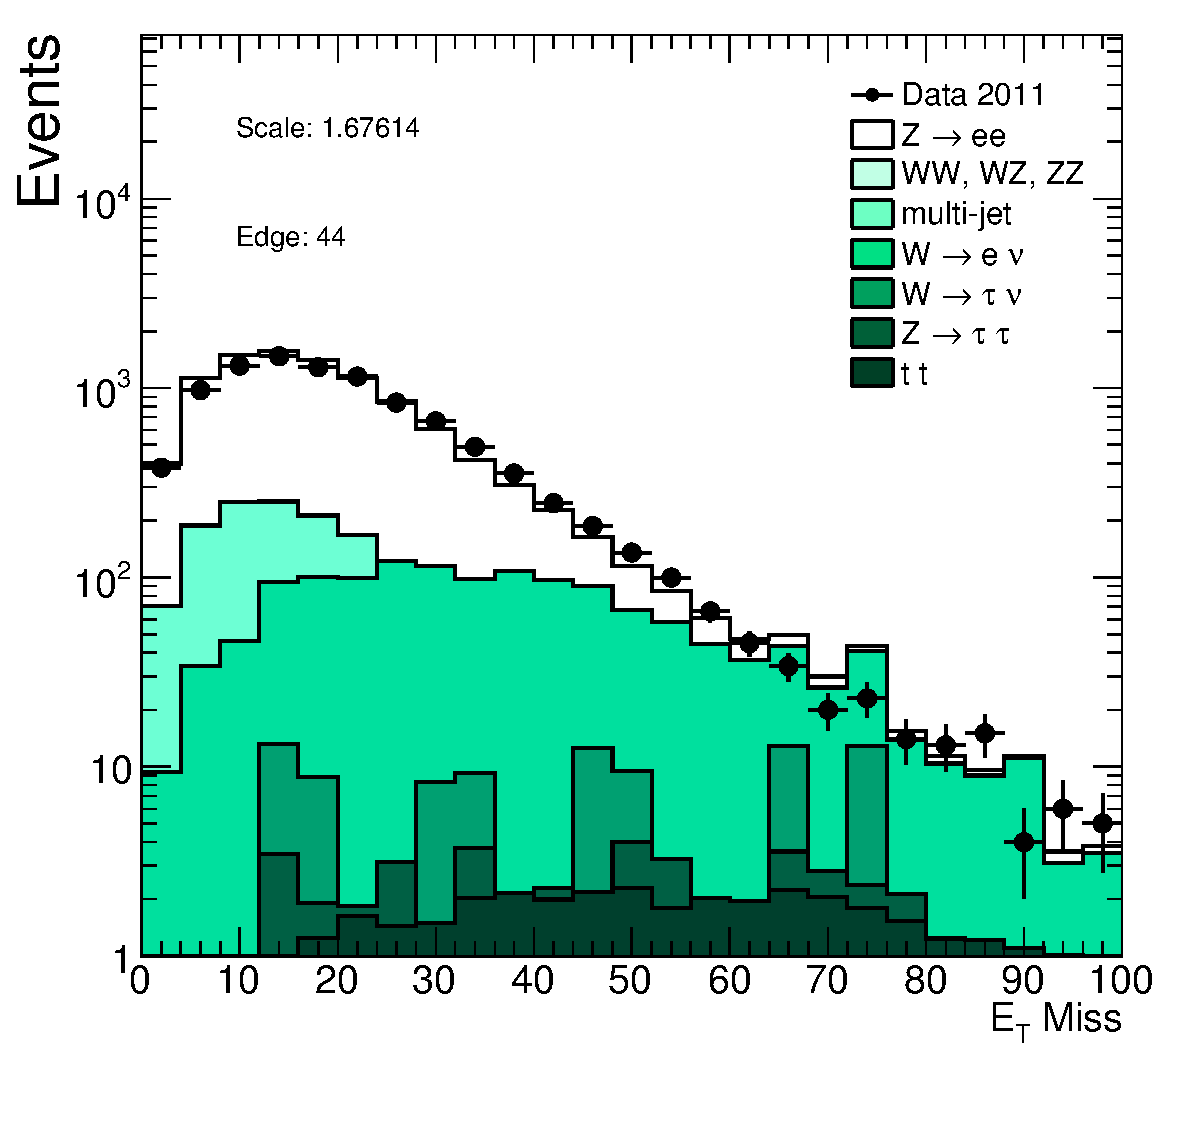
\includegraphics[width=0.32\textwidth]{figures/bkg_wenu_1.pdf}}
\subfigure[Mass window, $E_{t}^{miss}$]  {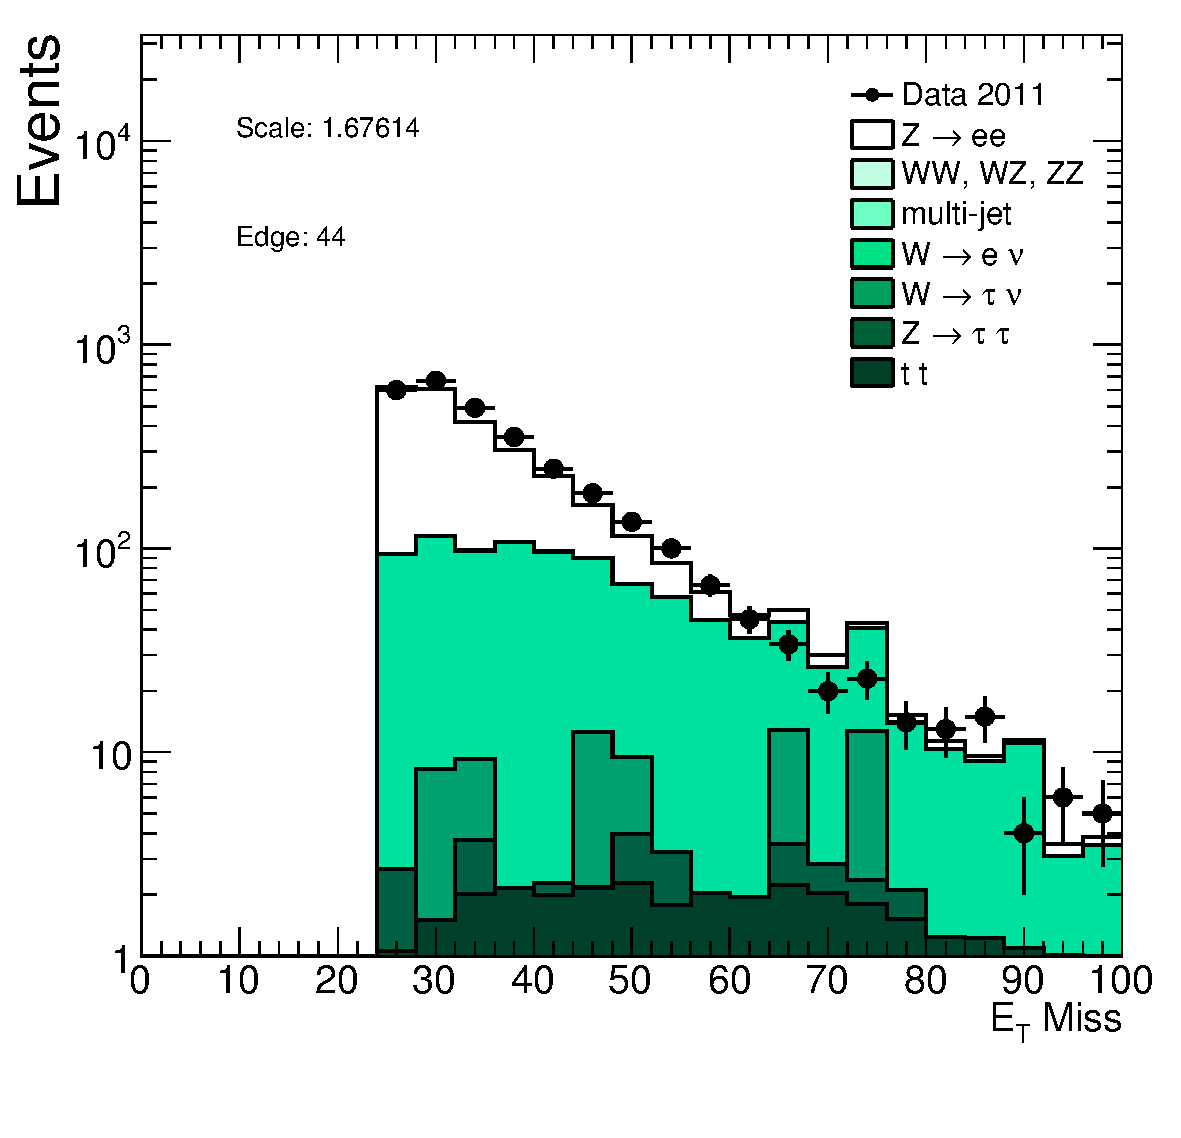
\includegraphics[width=0.32\textwidth]{figures/bkg_wenu_2.pdf}}
\subfigure[Mass window, $E_{t}^{miss}$, $M_{t}$] {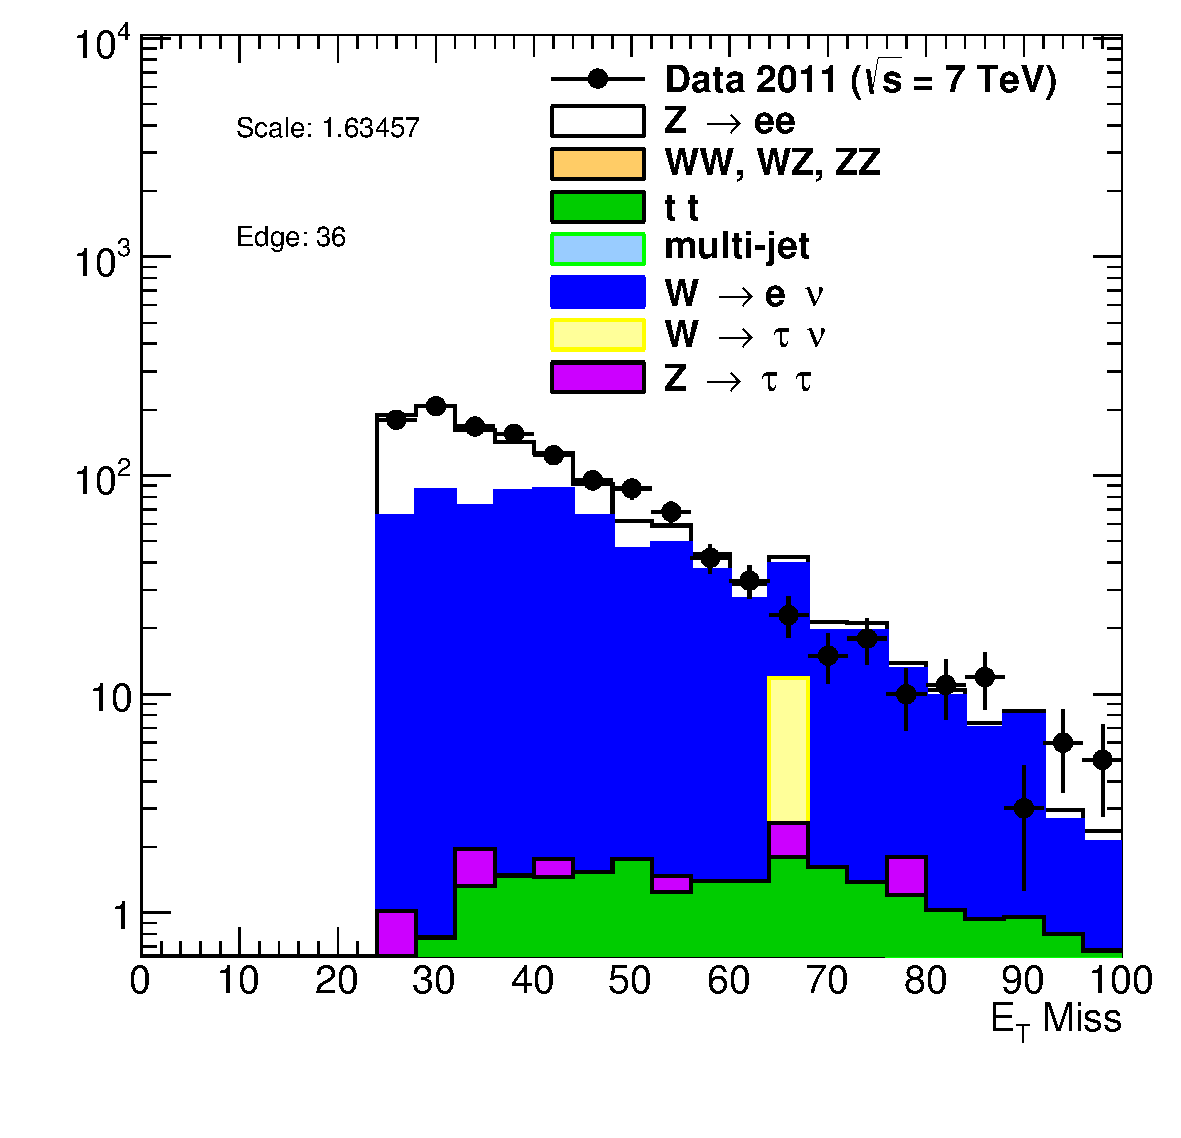
\includegraphics[width=0.32\textwidth]{figures/bkg_wenu_3.pdf}}

\caption{The data-fitting of the \Wenu\ background with various selections. (a) Mass window selection, (b) Mass window and $E_{t}^{miss} > 25$~GeV, (c) Mass window, $E_{t}^{miss} > 25$~GeV and $M_{t} > 50$~GeV.}
\label{fig:bkg_wenu}}
\end{figure}

All other electroweak backgrounds are simply scaled to the theoretically predicted luminocity-derived values. The resulting values for the electroweak background can be seen in Tab.~\ref{tab:bkg_ew_peak} for the peak mass, and in Tab.~\ref{tab:bkg_ew_high} for the high mass.

\begin{table}
\centering
\begin{tabular}{ c cccccccc } \hline \hline
 $y_Z$ bin & $t\bar t$ & $W \to e\nu$ & $W \to \tau\nu$ &  $WW$ & $WZ$ & $ZZ$ & $Z \to \tau\tau$  & $\gamma\gamma \to ee$\\  \hline
 1.2 -  1.4 &   0.18 &   1.90 &   0.00 &   0.04 &   0.08 &   0.04 &   0.01 &   0.10 \\
 1.4 -  1.6 &   0.11 &   1.61 &   0.38 &   0.03 &   0.07 &   0.03 &   0.06 &   0.09 \\
 1.6 -  1.8 &   0.08 &   1.10 &   0.10 &   0.03 &   0.05 &   0.03 &   0.09 &   0.08 \\
 1.8 -  2.0 &   0.06 &   1.03 &   0.00 &   0.02 &   0.04 &   0.02 &   0.06 &   0.07 \\
 2.0 -  2.2 &   0.04 &   0.87 &   0.03 &   0.02 &   0.04 &   0.02 &   0.08 &   0.05 \\
 2.2 -  2.4 &   0.03 &   0.75 &   0.10 &   0.02 &   0.04 &   0.02 &   0.10 &   0.05 \\
 2.4 -  2.8 &   0.01 &   0.65 &   0.13 &   0.02 &   0.04 &   0.02 &   0.11 &   0.05 \\
 2.8 -  3.2 &   0.00 &   0.35 &   0.08 &   0.01 &   0.02 &   0.01 &   0.08 &   0.04 \\
 3.2 -  3.6 &   0.00 &   0.05 &   0.00 &   0.00 &   0.01 &   0.01 &   0.01 &   0.03 \\
\hline \hline
\end{tabular}
\caption{Components of the electroweak background  in \% of selected data for $66 < m_{ee} < 116$~GeV.}
\label{tab:bkg_ew_peak}
\end{table}

\begin{table}
\centering
\begin{tabular}{ c cccccccc } \hline \hline
 $y_Z$ bin & $t\bar t$ & $W \to e\nu$ & $W \to \tau\nu$ &  $WW$ & $WZ$ & $ZZ$ & $Z \to \tau\tau$  & $\gamma\gamma \to ee$\\  \hline
 1.2 -  1.6 &   2.17 &  22.40 &   0.00 &   0.64 &   0.30 &   0.04 &   0.61 &   0.98 \\
 1.6 -  2.0 &   1.22 &  17.06 &   1.70 &   0.64 &   0.22 &   0.04 &   0.52 &   0.98 \\
 2.0 -  2.4 &   0.62 &   9.98 &   1.30 &   0.39 &   0.15 &   0.03 &   0.19 &   0.67 \\
 2.4 -  2.8 &   0.21 &   8.12 &   0.00 &   0.24 &   0.10 &   0.03 &   0.25 &   0.52 \\
 2.8 -  3.2 &   0.07 &   3.14 &   0.00 &   0.14 &   0.07 &   0.01 &   0.00 &   0.53 \\
 3.2 -  3.6 &   0.00 &   0.00 &   0.00 &   0.00 &   0.03 &   0.00 &   0.00 &   0.29 \\
\hline \hline
\end{tabular}
\caption{Components of the electroweak background in \% of selected data for $116 < m_{ee} < 150$~GeV.}
\label{tab:bkg_ew_high}
\end{table}

\section{QCD background}

The QCD background is the name for the multi-jet hadronic background. Since it's nearly impossible to simulate all the multitude of the hadronic processes with even remote accuracy. There are two methods to evaluate the amount of the multi-jet background. The first one is by using the theoretical functions to evaluate the form of the background. Usually the convolution of the Crystal Ball and the Breit-Wigner functions is used with the use of the RooFit framework~\cite{lib:bkg_roofit}. The second method is more precise and is usually used when the data samples are large enough to provide the adequate statistical error, and consist of constructing the background template (i.e. the form) from the data itself, by using the cut inversion: several cuts in the selection chain (usually the most basic ones) are inverted to provide the sample of the background events with the most "signal-like" signature. The amount of such events is usually very limited, but the total amount of the 2011 data allows us to use this method, which is otherwise better than the theoretical predictions of the RooFit method.

In both cases, after the template is constructed, it is normalized to the data, which is done by using the discriminatory variable. This variable shows how much background there is in any particular bin, to distinguish background-dominated bins from the signal-dominated bins. For the \Zee\ CF analysis the discriminatory variable was the isolation of the central electrone cluster $E_{t}^{\mathrm{cone30}}$. This variable showed the best results among the other tested, but since it is used in the default analysis selection, it can't be used direclty, and the background was normalized to the selection without the isolation cuts, and then scaled accordingly.

The background template is constructed based on the three selections: the one with the default cuts, with the default cuts and relaxed track and cluster isolation, and with the default cuts and relaxed cluster isolation only. For all selection the cut inversion included some of the electron tight ID criteria. See Tab.~\ref{tab:bkg_qcd_samples}. To calculate the systematic uncertainties for the background additional selections must be constructed. These selections must take into account the way the background is scaled: it is matched to the data in high-$E_{t}^{\mathrm{cone30}}$ bin, and the isolation cuts are not applied. See Tab.~\ref{tab:bkg_qcd_unc_samples} for the list.

\begin{table}
\centering
\begin{tabular}{ llll } \hline \hline
    & Cut inversion  &   Base selection    & expected bkg  \\ \hline
default & FwdTight, Tight++ & Default  & isolated \\
$S_1$   & FwdTight, Tight++ & Default w/o calo and track iso & all \\
$S_2$   & FwdTight, Tight++ & Default w/o calo iso       & $P_{t}^{\mathrm{cone}}$ isolated\\
\hline \hline
\end{tabular}
\caption{Event selections for QCD background estimation.}
\label{tab:bkg_qcd_samples}
\end{table}
\begin{table}
\centering
\begin{tabular}{ lll@{ w/o }ll } \hline \hline
    & Cut inversion  &  \multicolumn{2}{l}{Base selection}    & expected bkg \\ \hline
default\_1 & Tight++     & Default & FwdTight  & isolated \\
$S_2$\_1     & Tight++     & $S_1$ & FwdTight      & all \\
default\_2 & FwdMedium++ & Default & Tight++   & isolated \\
$S_2$\_2     & FwdMedium++ & $S_1$ & Tight++       & all \\
\hline \hline
\end{tabular}
\caption{Event selections for QCD background systematic uncertainties calculation.}
\label{tab:bkg_qcd_unc_samples}
\end{table}

The normalization procedure was made in several iterations, during which the background template and the signal MCs were scaled together to fit the data best, until the MC signal scalefactor is stabilized. Step by step explanation of the procedure is this:
\begin{itemize}
\item template is scaled to data based on the isolation tail bins: $s_{\mathrm{temp}} = \frac{N_{\mathrm{data}}^{\mathrm{tail}} - (s_{\mathrm{sig}} \cdot N_{\mathrm{sig.MC}}^{\mathrm{tail}}+N_{\mathrm{EWbkg}}^{\mathrm{tail}})}{N_{\mathrm{temp}}^{\mathrm{tail}}}$, where
\begin{itemize}
\item $s_{\mathrm{temp}}$ is the scalefactor for the QCD template;
\item $s_{\mathrm{sig}}$ is the scalefactor for the signal MC, which is $1.0$ at the first step;
\item $N_{\mathrm{data}}^{\mathrm{tail}}$ is the data events integrated over the isolation tail bins;
\item $N_{\mathrm{sig.MC}}^{\mathrm{tail}}$ is the signal MC events integrated over the isolation tail bins;
\item $N_{\mathrm{EWbkg}}^{\mathrm{tail}}$ is the electroweak background MC events integrated over the isolation tail bins;
\item $N_{\mathrm{temp}}^{\mathrm{tail}}$ is the template events integrated over the isolation tail bins;
\end{itemize}
\item the scaled template (i.e. the QCD background) is substracted from the data togethe with the electroweak background, and the remaining events are compared to signal MC to determine the new scalefactor for the MC: $s_{\mathrm{sig}} = \frac{N_{\mathrm{data}} - (s_{\mathrm{temp}} \cdot N_{\mathrm{temp}} + N_{\mathrm{EWbkg}})}{N_{\mathrm{sig.MC}}}$, where all the variables are the same, only integrated over all bins, not only the tail bins;
\item if the new MC scalefactor differs from the previous by less then $0.1$\%, the template scalefactor is considered to be final, otherwise, the new iteration is made.
\end{itemize}

For the systematic uncertainties, several values were used as the threshold of the tail region. For the central values, the template $S_{1}$ with $E_{t}^{\mathrm{cone30}}$ was chosen, as the one with the clearer separation of the background-dominated bins, and the most stable fit. The resulting QCD background estimations can be seen in Figs.~\ref{fig:bkg_qcd} and in Tabs.~\ref{tab:bkg_qcd_peak_percents} and~\ref{tab:bkg_qcd_high_percents}.

\begin{figure}
\center{
\subfigure[$66 < m_{ee} < 116$~GeV] {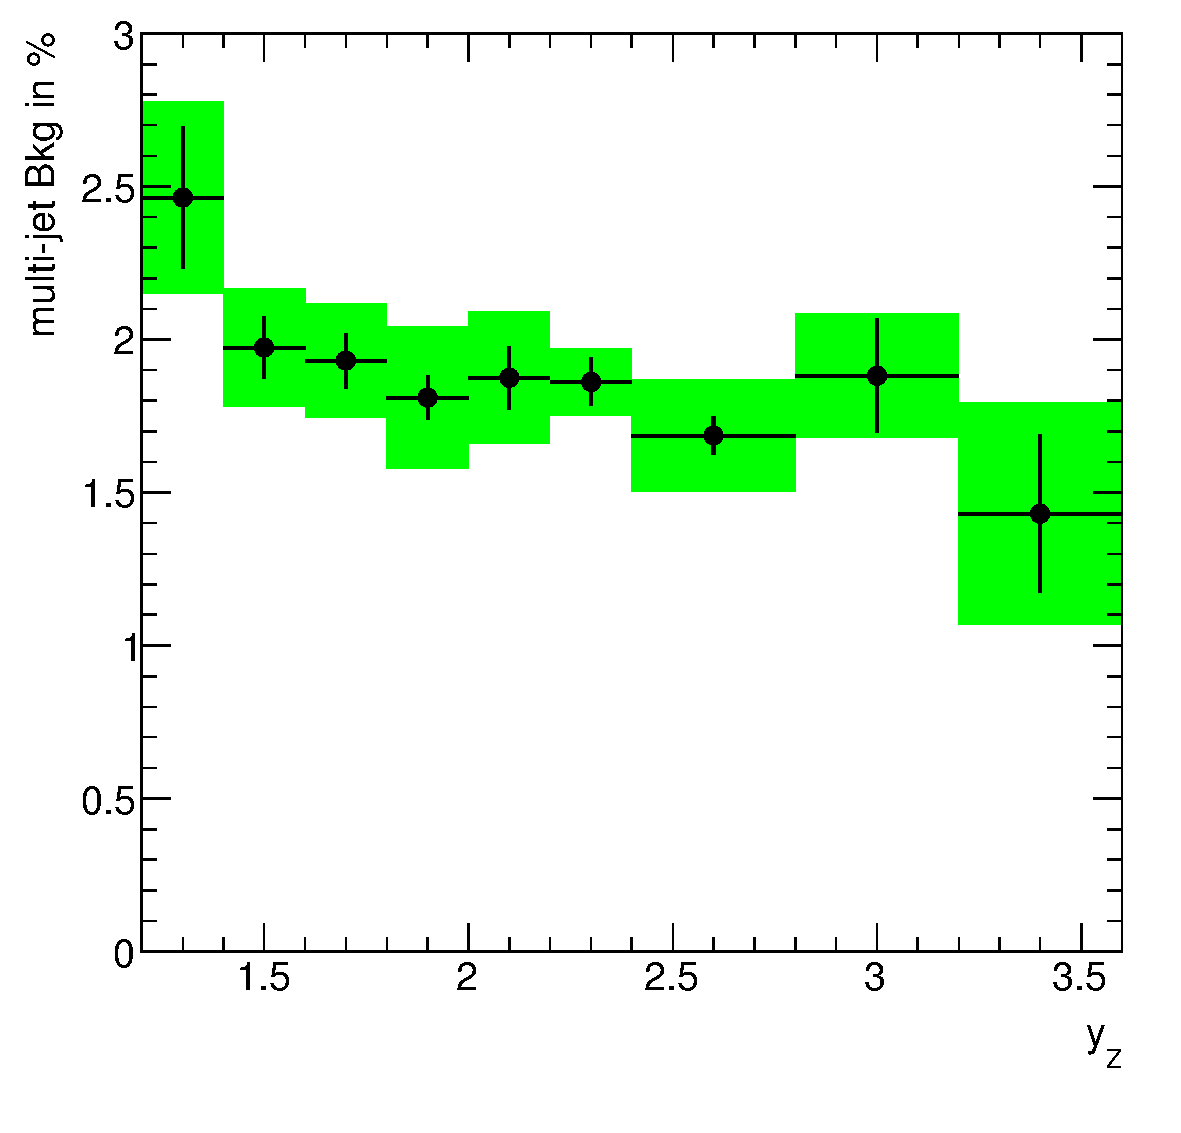
\includegraphics[width=0.45\textwidth]{figures/bkg_qcd_peak.pdf}}
\subfigure[$116 < m_{ee} < 150$~GeV]  {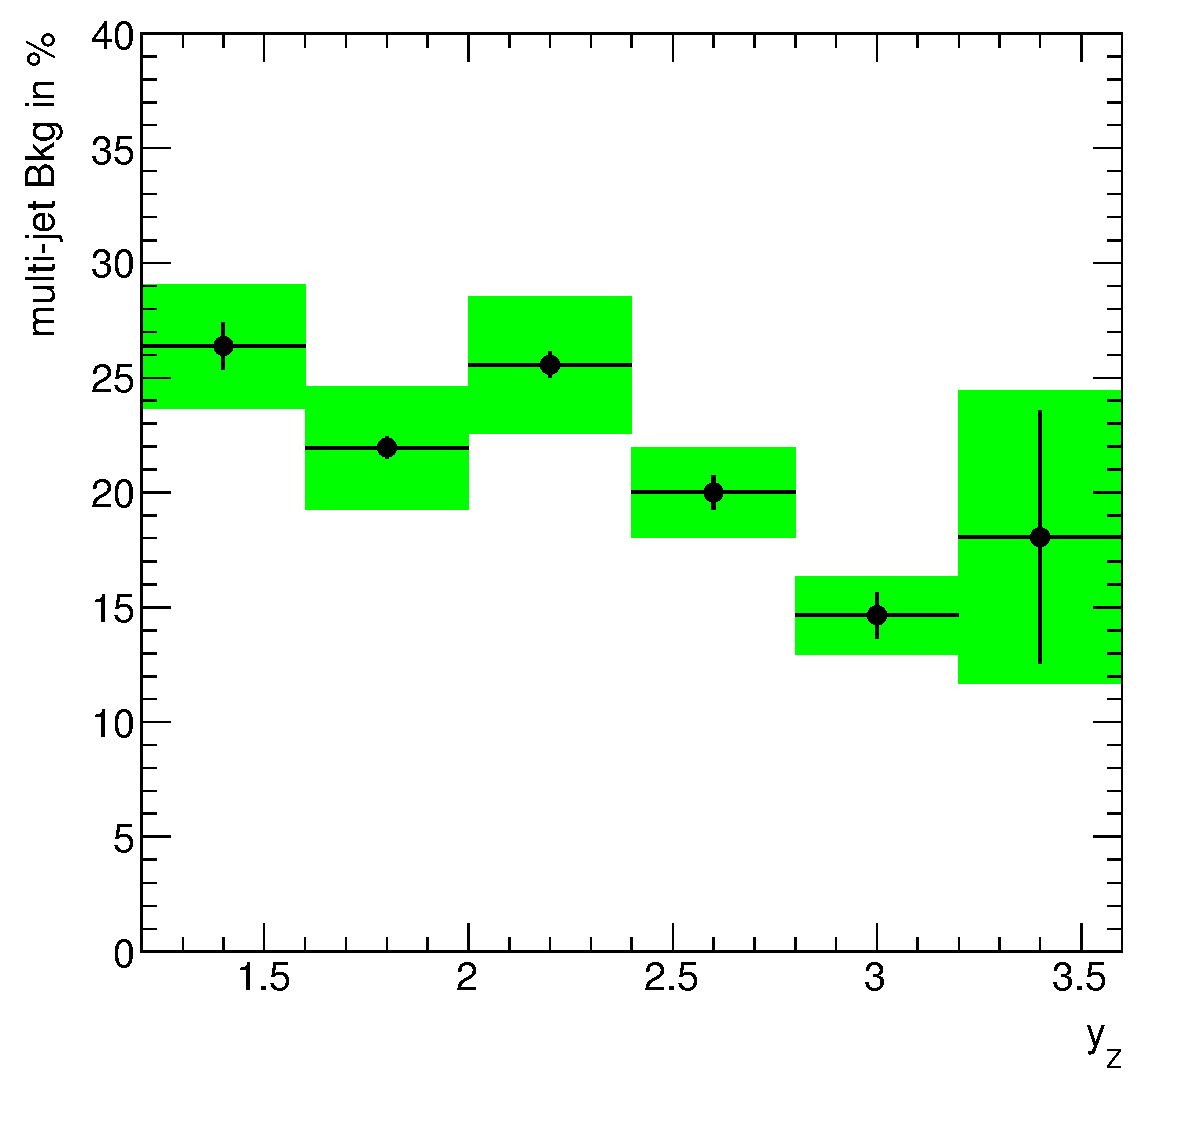
\includegraphics[width=0.45\textwidth]{figures/bkg_qcd_high.pdf}}
\caption{The QCD background estimation for the \Zee\ central-forward analysis, (a) for peak mass and (b) for high mass.}
\label{fig:bkg_qcd}}
\end{figure}

\begin{table}
\centering
\begin{tabular}{ cccc } \hline \hline
 $y_Z$ bin & QCD bkg & Stat & Syst \\  \hline
 1.2 -  1.4 &   2.46 &   0.23  &   0.21 \\
 1.4 -  1.6 &   1.97 &   0.10  &   0.16 \\
 1.6 -  1.8 &   1.93 &   0.09  &   0.16 \\
 1.8 -  2.0 &   1.81 &   0.07  &   0.22 \\
 2.0 -  2.2 &   1.87 &   0.10  &   0.19 \\
 2.2 -  2.4 &   1.86 &   0.08  &   0.07 \\
 2.4 -  2.8 &   1.69 &   0.06  &   0.17 \\
 2.8 -  3.2 &   1.88 &   0.19  &   0.08 \\
 3.2 -  3.6 &   1.43 &   0.26  &   0.25 \\
\hline \hline
\end{tabular}
\caption{The bin-by-bin QCD background astimation for the \Zee\ CF $66 < m_{ee} < 116$~GeV analysis in percents.}
\label{tab:bkg_qcd_peak_percents}
\end{table}

\begin{table}
\centering
\begin{tabular}{ cccc } \hline \hline
 $y_Z$ bin & QCD bkg & Stat & Syst \\  \hline
 1.2 -  1.6 &  26.37 &   1.04  &   2.50 \\
 1.6 -  2.0 &  21.96 &   0.47  &   2.63 \\
 2.0 -  2.4 &  25.57 &   0.57  &   2.95 \\
 2.4 -  2.8 &  20.00 &   0.72  &   1.84 \\
 2.8 -  3.2 &  14.64 &   1.01  &   1.36 \\
 3.2 -  3.6 &  18.07 &   5.53  &   3.17 \\
\hline \hline
\end{tabular}
\caption{The bin-by-bin QCD background astimation for the \Zee\ CF $116 < m_{ee} < 150$~GeV analysis in percents.}
\label{tab:bkg_qcd_high_percents}
\end{table}
